% \documentclass[10pt]{scrartcl}
\documentclass[10pt,twocolumn]{scrartcl}

\usepackage[utf8]{inputenc}
\usepackage[T1]{fontenc}
\usepackage[ngerman]{babel}

\usepackage{amsmath}
\usepackage{amssymb}

\usepackage{graphicx}
\usepackage{tabularx}
\usepackage{authoraftertitle}

\setlength{\parindent}{0cm}
\setlength{\parskip}{3mm}
\setlength{\textheight}{23.8cm}
\setlength{\headheight}{1cm}
\setlength{\topmargin}{-10mm}

\setlength{\oddsidemargin}{0cm}
\setlength{\evensidemargin}{0cm}
\setlength{\textwidth}{16cm}
\setlength{\columnsep}{8mm}

\usepackage{multicol}
\usepackage{colortbl}
\usepackage{xcolor}
\definecolor{grau}{gray}{0.95}
\definecolor{dunkelgrau}{gray}{0.85}

\usepackage[normal]{caption}
\usepackage{lipsum}

\setlength{\parindent}{5mm}
\setlength{\parskip}{0mm}

\usepackage{float}
\restylefloat{figure}

\renewcommand{\topfraction}{0.75}
\renewcommand{\textfraction}{0.2}

%###########################################################
% die Sachen mit der Kopfzeile
\usepackage{lastpage}
\usepackage{fancyhdr}
\fancyhf{} % leere alle Felder
\fancyhead[R]{\footnotesize Phillip Schichtel: phillip.dhbw@schich.tel \\ Jonas Dann: jonas.chr.dann@gmail.com}
\fancyhead[L]{\footnotesize Ausgewählte Methoden der
Datenanalyse, \\ Modellierung und Simulation - Raytracing} % Titel des Aufsatzes
\fancyfoot[C]{\footnotesize \thepage/\pageref{LastPage}}
% \fancyfoot[C]{\footnotesize \thepage}
\renewcommand{\headrulewidth}{0.4pt} % obere Trennlinie
\pagestyle{fancy}
%###########################################################

\title{Raytracing - Schattenberechnung im zweidimensionalen Raum}

\newcommand{\ownsection}[1]{\begin{center}\LARGE\bf#1\end{center}}

\begin{document}


{
  \onecolumn
  \maketitle
}

{
  \onecolumn
  \tableofcontents
}

\twocolumn[
\ownsection{\MyTitle}

\begin{center}
Phillip Schichtel (phillip.dhbw@schich.tel) \\
Jonas Dann (jonas.chr.dann@gmail.com) \\
Mannheim, Oktober 2014
\end{center}
\vspace*{5mm}
]

% \begin{multicols}{2}
\section{Abstract}

Im Folgenden werden verschiedene Methoden zur Simulation von realistischen Schatten
vorgestellt und diskutiert. Dabei werden die Verfahren ``Shadow Mapping'',
``Ray tracing'' und ``Shadow Volumes'' theoretisch und die Implementierung
einer Abwandlung des ``Shadow Volumes''-Verfahrens praktisch gezeigt.


\section{Einleitung \& Motivation}

Schatten gibt es überall, wo es Licht gibt. Dies gibt es zu bedenken, wenn
Gebäude oder außenbereiche geplant werden.
Desweiteren verleihen Schatten flachen Objekten eine gewisse Tiefe für das menschlische Auge.
Dies wird genutzt um in Filmen digital eingefügte Objekte realistisch aussehen zu lassen.

Aber auch in Spielen werden Schatten auf die verschiedensten Weisen verwendet, dort werden
die Schatten meistens auch in Echtzeit berechnet da sich die Spielwelten in den meisten Spielen
ständig ändern.

Architekten nutzen Licht- und Schattensimulationen um Räume zu planen, bei denen eine passende
Ausleuchtung essentiell ist.

\subsection{Anwendung in Spielen}

In Spielen trifft man auf viele verschiedene Anwendungen von Licht und Schatten. In den meisten
Spielen werden die Schatten genutzt, um die Spielwelt realistischer und glaubwürdiger darzustellen.
Dabei treten häufig viele verschiedene Lichtquellen in einer Szene auf, was für die Berechnung der
Schatten sehr effiziente Algorithmen benötigt, denn eine Szene (ein Bild) muss für eine Bildrate
von 60 $\frac{\text{Bilder}}{\text{Sekunde}}$ in unter 16 Millisekunden fertig von der Grafikkarte gezeichnet sein.

Zum Zeitpunkt der Veröffentlichung dieser Arbeit ist es üblich, grobe Annäherungen zu verwenden,
wie sie etwa durch das ``Shadow Mapping''-Verfahren berechnet werden.

Andere Spiele verwenden ähnliche Berechnungen auch für Spielelemente. So wird in dem Spiel ``Monaco'' \cite{monaco2014},
ein 2D Spiel in der Vogelperspektive, der Spieler als gerichtete Lichtquelle betrachtet um verdeckte
Elemente, also Elemente im Schatten des Blicks, auszublenden.

\subsection{Anwendung in der Architekur}

Architekten simulieren bei neu entworfenen Gebäuden auch den Lichteinfall zu verschiedenen Tageszeiten.
Das ist besonders dann wichtig, wenn Kunden gut ausgeleuchtete Räume wollen oder auch wenn es darum geht
Sitzmöglichkeiten auf Plätzen zu planen. In ersterem will man die Schatten durch geschickte Platzierung
von Fenstern und Lampen minimieren, bei letzterem will man den Schatten zu bestimmten Tageszeiten
möglichst lange halten.

\subsection{Anwendung in Filmen}

Viele Szenen in modernen Filmen werden heutzutage vollständig am Computer generiert. Damit diese Szenen
real aussehen, müssen auch hier wie bei den Spielen akurate Schatten berechnet werden.

\section{Problemstellung und Methoden}

\subsection{Umbra, Penumbra und Antumbra}

In der Theorie von Schatten wird ein Schatten in 4 Teile zerlegen.
\begin{enumerate}
 \item \emph{Umbra}, der Kernschatten, ist der Teil des Schattens der von keinerlei Licht erreicht wird.
       Wenn es nur eine Lichtquelle gibt, dann hat jeder Schatten einen Umbra.
 \item \emph{Antumbra}, der weiche Schatten, der hinter dem Umbra entsteht. Dieser Bereich entsteht nur,
       wenn die Lichtquelle größer ist, als das Objekt, dass den Schatten wirft. Der Antumbra beginnt an
       dem Punkt, an dem das Objekt die Lichtquelle nicht mehr vollständig verdecken kann und man die
       Ränder der Lichtquelle sehen kann.
 \item \emph{Penumbra}, die zwei weichen Schatten, die an den Seiten des Umbras entstehen. Diesen Bereich
       gibt es immer, wenn der Schatten nicht von einer Punktlichtquelle geworfen wird, in der realen
       Welt als immer. In diesem Bereich beginnt man die Seite der Lichtquelle zu sehen, die vorher im
       Umbra verdeckt wurde.
\end{enumerate}
Diese 3 separaten Bereiche eines Schatten sollten optisch realistisch dargestellt werden können.
Damit gilt also als Anforderung, dass Lichtquellen simuliert werden können, die eine Breite haben
und nicht nur einfach ein Punkt sind.


\subsection{Shadow Mapping}

Schatten abbilden

\subsection{Raytracing}

Strahlen verfolgen

\subsection{Shadow Volumes}

Schatten zum Würfel

In naturwissenschaftlichen Veröffentlichungen sollte immer 
ein 'Abstract', eine 'Einleitung' und soetwas wie 'Ergebnisse und
Diskussion' vorhanden sein. Andererseits muss man sich bei den
Abschnitten wie 'Material und Methoden' und der 'Durchführung'
nicht zwingend an die Überschriften halten. 

Wichtig ist nur, dass man eingehens die Mittel, Techniken,
Methoden, vielleicht das mathematische Instrumentarium 
oder den experimentelle Aufbau erwähnt, mit welchem man 
gearbeitet hat und was essentiell zum Verständnis sein könnte.

Wenn Sie den Leser vorbereitet haben, was da kommt, dann können
Sie die große Synthese startet und ihr ganzes Setup mit allen
nötigen Parametern beschreiben, aus denen Sie letztendlich
die Ergebnisse generiert haben. Aus diesen Überlegungen heraus, 
sieht man bereits, dass die Grenzen zwischen den Bereichen 
'Material und Methoden' sowie 'Durchführung' und mitunter 
bis zu den 'Ergebnissen' verschwimmen können.

\subsection*{Ideen zum Lesen aus der Sicht eines Massenkonsumenten}

Da heutzutage enorm viele wissenschaftliche Artikel
eingereicht und veröffentlich werden, und das in zig verschiedenen
Journalen, kann niemand alles lesen und nur wenige haben die Zeit 
sehr viel zu lesen. Und da man als Leser noch andere Dinge im Leben 
vorhat, gibt es ein paar Techniken.
Diese Techniken spiegeln auch ein wenig die Bedeutung der einzelnen 
Abschnitte einer Veröffentlichung wieder.

Das Wichtigste ist natürlich die Überschrift, denn wenn diese außerhalb
der Interessensphäre des Lesers liegt, dann wird der Leser weiter suchen
und eine anderen Artikel heranziehen.

Danach wendet sich der Vielleser dem Abstract zu. Wenn dieses spannend ist,
wird dieser der Veröffentlichung mehr Zeit widmen. In Fächern wie der
Biochemie gibt es sogar Leute, die nur die Abstracts lesen, was durchaus
seine Berechtigung hat. Im diesen Abstracts stehen beispielsweise, 
wie bestimmte Proteine reagieren. Meistens ist das ausreichend für 
die eigene Forschung oder um etwas in Erfahrung zu bringen.
Übrigens sollte man im Internet theoretisch zu allen Veröffentlichung
die Abstracts mit dem Titel und den Autoren finden, die seit Anbeginn 
elektronischer Journals eingereicht wurden. Bei kostenpflichtigen 
Journals ist das Abstract wie der der Klappentext beim Buch und
entscheidet über Kauf oder Nichtkauf.

Die Diskussion könnte man als dritte Anlaufstelle nehmen. Wenn Sie 
die Ergebnisse, die im Abstract vielleicht bahnbrechend wirkten, genau 
beleuchtet wissen wollen, so sollten Sie hier mehr darüber
finden. Als Autor müßte man sich an dieser Stelle entsprechend 
kritisch mit den Ergebnissen auseinandersetzen. Auch ein Ausblick
ist manchmal sehr nett.

Als Viertes findet man noch eine hohe Informationsdichte in
Abbildungen, Diagrammen und Tabellen. Diese müssen so präsentiert werden,
dass man nicht hunderte von Zeilen Text durchforsten muss, damit man Sie versteht.
Dementsprechend braucht es eine Unterschrift bei Abbildungen und Diagrammen 
und einer Überschrift bei Tabellen wie es am Beispiel von Tab.~\ref{tab:falsch}
gezeigt wird. Achsenbeschriftungen, Einheitenangaben
und generell Übersichtlichkeit ist selbstredend zu beachten.
Andernfalls wird der Autor vielleicht als stümperhaft oder mindestens
wenig beflissentlich wahrgenommen.

\begin{table}[t]
\caption{Eine auffällig gefälschte Statistik über die Wissensaufnahme $\xi$
(in Wissenseinheit pro Minute) in Abhänigkeit von der verstrichenen Vorlesungszeit.}
\label{tab:falsch}
\centering
\begin{tabular}{cc}
\rowcolor{dunkelgrau}
Zeit [min] & $\xi$ [WE/min] \\
0 - 15 & 20 \\
\rowcolor{grau}
15 - 30 & 30 \\
30 - 45 & 42 \\
\rowcolor{grau}
45 - 60 & 70 \\
60 - 75 & 50 \\
\rowcolor{grau}
75 - 90 & 84
\end{tabular}
\end{table}

Wenn nun all das für den Leser interessant wirkte und dieser es vielleicht
selber im Detail nachvollziehen möchte, dann wird er sich wahrscheinlich
dem restlichen Text widmen.

Natürlich ist das eben Geschriebene nur eine Ideenskizze und wenn
Sie eine andere Herangehensweise an das Lesen solcher Artikel haben,
so steht dies Ihnen selbstverständlich frei.

\section{Durchführung}

Das verwendete Verfahren spiegelt ein Shadow Volumes artiges Verfahren im zweidimensionalen Raum wieder. Auch hier wird die Silhouette des angestrahlten Rechtecks berechnet und and die Grenzen, des Fensters auf dem Bildschirm, projiziert. Der von dieser Projektion abgedeckte Bereich wird dunkler eingefärbt.

Der Rasterizer, welche die Schattenfläche auf die Lichtwerte der Pixel in dem Fenster anwendet, benötigt zwei Strahlen, welche die Projektion der Silhouette darstellen, und ein Array von Punkten welche alle Eckpunkte des Rechtecks, welche auf der dunklen Seite des Objektes liegen, enthält. Diese werden benötigt, damit der Schatten das Rechteck nicht teilweise bis ganz überdeckt. Somit kann man die Objekte in der Szene besser voneinander unterscheiden und sieht nicht ausschließlich schwarze Flächen.

Es wird vor jeder Berechnung der Schatten von einem vollkommen beleuchteten Raum ausgegangen. Dazu wird für jeden Pixel auf dem Bildschirm der Wert 1, von allen Lichtquellen beleuchtet, gespeichert.

%\begin{figure}[t]
%	\centering
%	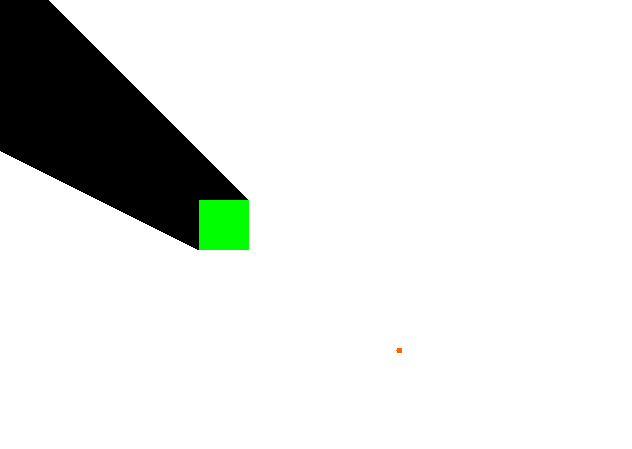
\includegraphics[width=\columnwidth]{images/durchfuehrung.png}
%	\caption{einfacher Schatten}
%	\label{fig:durch1}
%\end{figure}

Im Folgenden wird die entwickelte Methode gezeigt um einen Schatten zu berechnen, wie er zum Beispiel in Abbildung \ref{fig:durch1} zu sehen ist.

%\begin{figure}[t]
%	\centering
%	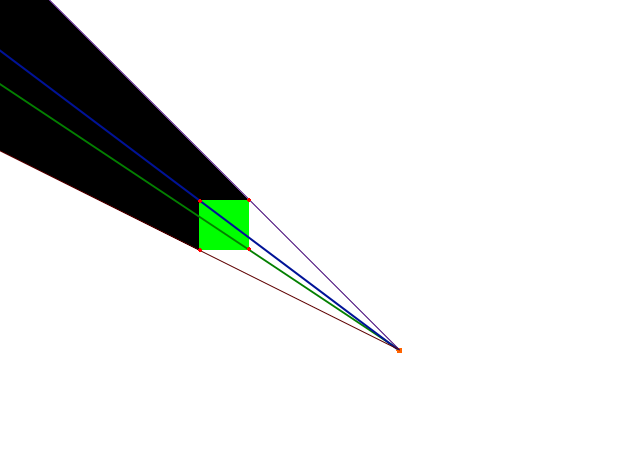
\includegraphics[width=\columnwidth]{images/durchfuehrung_1.png}
%	\caption{Geraden durch Eckpunkte}
%	\label{fig:durch2}
%\end{figure}

Im ersten Schritt der Berechnung werden durch jeden Eckpunkt 
\begin{equation}
	P = \left(\begin{array}{c} p_1 \\ p_2 \end{array}\right)
\end{equation}
des schattenwerfenden Objektes und die Lichtquelle
\begin{equation}
	L = \left(\begin{array}{c} l_1 \\ l_2 \end{array}\right)
\end{equation}
Geraden 
\begin{equation}
	\vec{g} = \left(\begin{array}{c} p_1 \\ p_2 \end{array}\right) + r * \left(\begin{array}{c} p_1 - l_1 \\ p_2 - l_2 \end{array}\right)
\end{equation}
gelegt (Abbildung \ref{fig:durch2}).

%\begin{figure}[t]
%	\centering
%	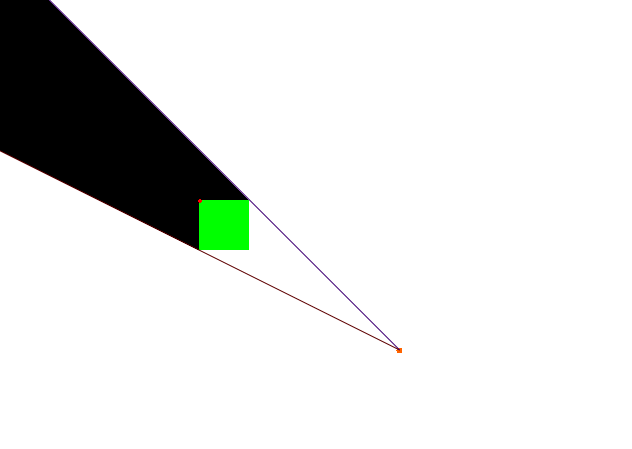
\includegraphics[width=\columnwidth]{images/durchfuehrung_4.png}
%	\caption{Geraden mit größtem Winkel}
%	\label{fig:durch3}
%\end{figure}

%\vec{e}_1=\left(\begin{array}{c} 1 \\ 0 \end{array}\right)

Ausschlaggebend für den geworfenen Schatten sind die zwei Geraden, deren Winkel am weitesten auseinander liegt (Abbildung \ref{fig:durch3}). Dazu wird rekursiv jedes Geradenpaar 

\begin{equation}
	\vec{g}_1 = \vec{o}_1 + r * \vec{m}_1, \vec{g}_2 = \vec{o}_2 + s * \vec{m}_1
\end{equation}
durch den Winkel
\begin{equation}
	\omega = arccos(\vec{m}_1 * \vec{m}_2 / (|\vec{m}_1| * |\vec{m}_2|))
\end{equation}

mit dem vorherig größten Geradenpaar verglichen und das mit dem größeren Winkel zurückgegeben.

%\begin{figure}[t]
%	\centering
%	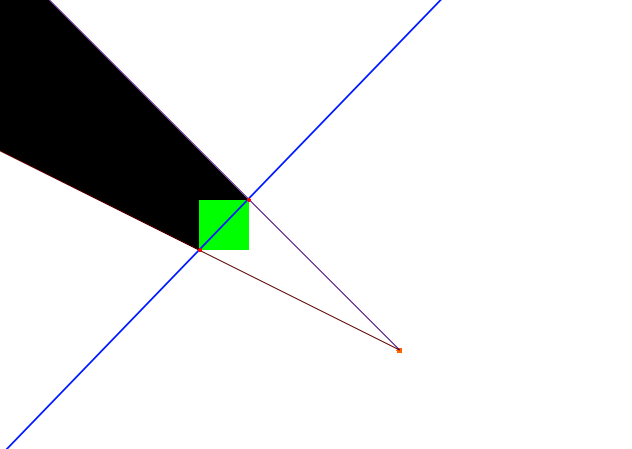
\includegraphics[width=\columnwidth]{images/durchfuehrung_2.png}
%	\caption{Gerade durch Ortsvektoren}
%	\label{fig:durch4}
%\end{figure}

Damit später die Objekte nicht vom eigenen Schatten teilweise bis ganz überdeckt werden, werden nun die Eckpunkte des Rechtecks berechnet, welche auf der dunklen Seite des Objektes liegen. Dazu wird eine Gerade durch die Ortsvektoren der zwei vorher bestimmten Geraden bestimmt (Abbildung \ref{fig:durch4}).

\begin{equation}
	s: \vec{s} = \vec{o}_1 + t * \left(\begin{array}{c} o_21 - o_11 \\ o_22 - o_12 \end{array}\right)
\end{equation}

%\begin{figure}[t]
%	\centering
%	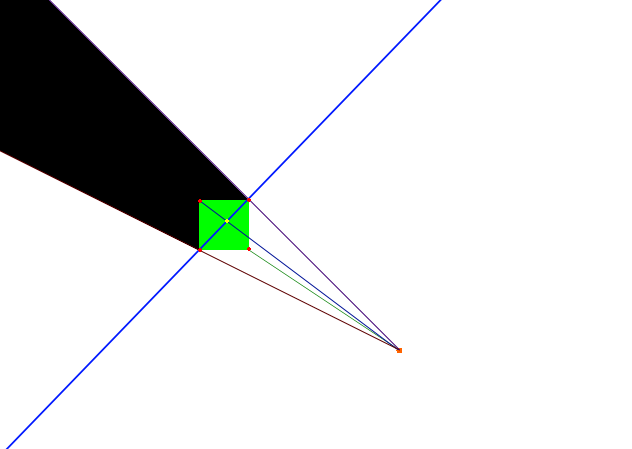
\includegraphics[width=\columnwidth]{images/durchfuehrung_3.png}
%	\caption{Eckpunkte auf der dunklen Seite}
%	\label{fig:durch5}
%\end{figure}

Wenn ein Schnittpunkt zwischen der Geraden $s$ und der Strecke zwischen einem Eckpunkt des Rechtecks und der Position der Lichtquelle vorhanden ist hängen wir diesen Eckpunkt an das an den Rasterizer zu übergebende Array an (Abbildung \ref{fig:durch5}).

\section{Ergebnisse und Diskussion}

%\begin{figure}[t]
%	\centering
%	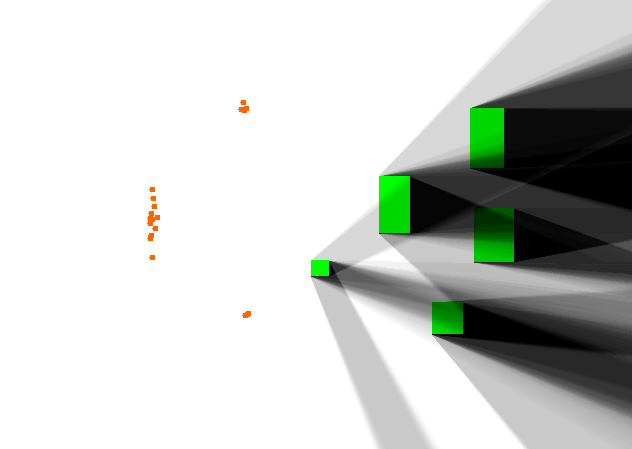
\includegraphics[width=\columnwidth]{images/ergebnis_4.png}
%	\caption{Ergebnis 1}
%	\label{fig:ergeb1}
%\end{figure}

%\begin{figure}[t]
%	\centering
%	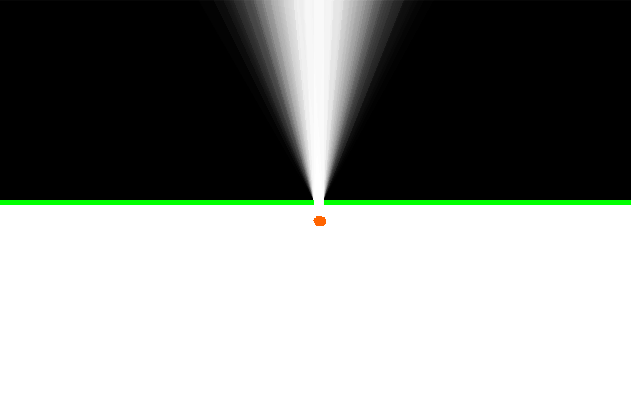
\includegraphics[width=\columnwidth]{images/ergebnis.png}
%	\caption{Ergebnis 2}
%	\label{fig:ergeb2}
%\end{figure}

%\begin{figure}[t]
%	\centering
%	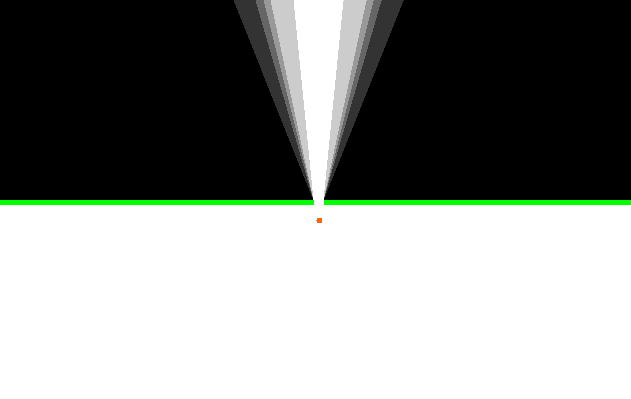
\includegraphics[width=\columnwidth]{images/ergebnis_2.png}
%	\caption{Ergebnis 3}
%	\label{fig:ergeb3}
%\end{figure}

%\begin{figure}[t]
%	\centering
%	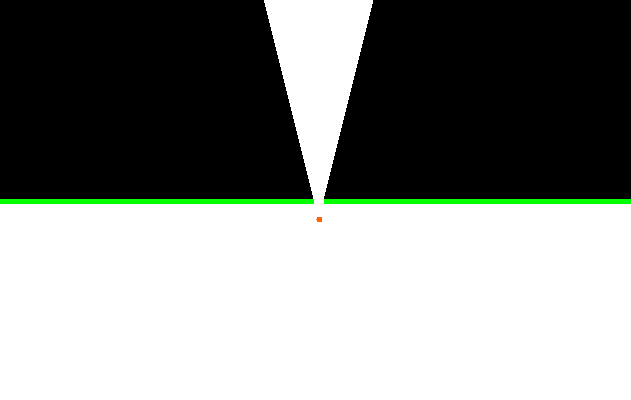
\includegraphics[width=\columnwidth]{images/ergebnis_3.png}
%	\caption{Ergebnis 4}
%	\label{fig:ergeb4}
%\end{figure}

Was Sie hier finden sollten, findet sich leider schon in den vorangegangenen
Textpassagen und Abschnitten und ich mag Sie nicht mit Wiederholungen
langweilen. Jedoch kann man ab und zu feststellen, dass das Abstract und
die Diskussionen eine gewisse Ähnlichkeit aufweisen, wobei die Diskussion
immer ausführlicher sein soll. Das liegt mitunter daran, dass beide 
Abschnitte Zusammenfassungen mit unterschiedlicher Nuancierung darstellen. 

Jetzt möchte ich mich gleich auf genau dieses Schreiben beziehen, 
von dem ich hoffe, dass Sie hinsichtlich des Schreibens und Lesens 
von solchen Ideen- und Gedankenmanifestationen etwas für sich mitnehmen konnten. 
Selber hatte ich mit diesem Thema verstärkt während meiner Doktorarbeit \cite{Gerhards2008} 
zu tun gehabt, ohne selber der enthusiastischste Leser gewesen zu sein.
Viele Ideen und Ansichten habe ich jedoch von meinem Doktorvater 
Prof. Dr. Kurt Roth mitbekommen, dessen arbeitsgruppeninterne Übungen 
zum schnellen Lesen förderlich für die Adrenalinproduktion waren.

% Ziel der Vorlesung war neben der sehr theorielastigen Einführung
% in die Fourier-Transformation, Faltung, Korrelationsanalyse und
% der nichtlinearen Optimierung, dass Sie sich mit einem Problem
% mit stark physikalischem Schwerpunkt auseinandersetzen sollten.
% Hier galt es sich einzuarbeiten und danach die entsprechenden
% Werkzeuge zum Lösen des Problems sowie zur graphischen Visualisierung
% anzueignen. Die Päsentation sowie der Abschlussbericht stellen
% dann die mündliche, wie schriftliche Darlegung des Problems und
% dessen Lösunng dar.
% 
% Und auch wenn Sie mit Ihrem Problem in Zukunft nie wieder in
% Berührung kommen werden, ist es generell wichtig Probleme anzugehen,
% die Werkzeuge zur dessen Bewältigung anzueignen und danach die
% Problemlösung auch voranzutreiben. Wissenschaftlichkeit in den
% Sachverhalt einfließen zu lassen, bedeutet dann noch das Problem
% in einem größeren Kontext zu sehen oder auch in Bezug auf verwandte
% Problematiken.

% Zum Abschluss aber noch einen Witz: Stellen Sie sich eine Party
% vieler mathematischer Funktionen vor. Auf einmal öffnet sich die
% Tür und ein Differentialoperator tritt herein. Alle Funktionen
% suchen die Flucht, nur die e-Funktion bleibt an der Bar stehen.
% Kommt der Differentialoperator zur e-Funktion und fragt, warum
% sie denn nicht weglaufen täte. 'Na, ich bin doch die Funktion e hoch x.
% Du kannst mich nicht wegdifferenzieren.' Darauf antwortet der
% Differentialoperator: 'Aber ich leite doch nach y ab.'

Schließen möchte ich mit einem Zitat von Wittgenstein \cite{Wittgenstein1922},
welches Prof. Dr. Kurt Roth im Zusammenhang wissenschaftlichen
Schreibens gerne nutzte: {\it Was sich überhaupt sagen lässt, lässt
sich klar sagen; und wovon man nicht reden kann, darüber muss man
schweigen.} 

\section{Diskussion}

Wenn es jemanden zu danken gibt, wie beispielsweise die Geldgeber, 
dann ist hier der Ort.

\subsection{Die Grenzen des gewählten Ansatz}

Ich für meinen Teil möchte den Dank an Prof. Dr. Tobias Straub
richten, für das Angebot eine Vorlesung an der Dualen Hochschule in
Mannheim halten zu dürfen. Auch einen Dank an all die Studenten der Vorlesung

\subsection{Alternative Ansätze}

und besonders für die spannenden Projekte, bei den ich teils auch 
etwas hinzulernen durfte. Am Ende nochmals vielen Dank 

\subsection{Abdeckung der Problematik}

an den bereits erwähnten Prof. Dr. Kurt Roth für alles, 
was ich während meiner Doktorarbeit durch ihn gelernt habe.

\begin{thebibliography}{99}
\bibitem{monaco2014}http://www.monacoismine.com/
\bibitem{Goos1947}F.Goos und H.Hänchen: {\it Ein neuer fundamentaler Versuch zur Totalreflektion}, 1947; Annalen der Physik 436, S. 333-346
\bibitem{Einstein1905}A.Einstein {\it Zur Elektrodynamik bewegter Körper}, 1905; Annalen der Physik und Chemie 17, S. 891-921
\bibitem{Gerhards2008}H.Gerhards: {\it Ground Penetrating Radar as a Quantative Tool with Applications in Soil Hydrology}, Heidelberg 2008; Dissertaton,
\bibitem{Wittgenstein1922}L.Wittgenstein: {\it Tractatus Logico-Philo\-so\-phi\-cus}, London 1922; Kegan Paul, Trench, Trubner \& Co., Ltd.
\end{thebibliography}

\end{document}
